\begin{question}
\Programming\ 
Consider a system as illustrated below.
%
\begin{center}
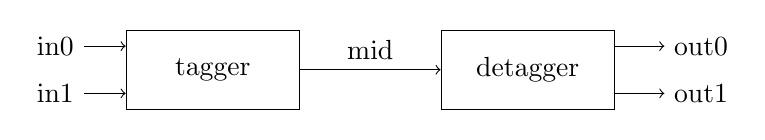
\begin{tikzpicture}
\draw(0,0) node[draw, minimum height = 10mm, minimum width = 22mm] 
  (tagger) {tagger};
\draw(-2,0) node (left){};
\draw ([yshift = 3mm] left) node (in0) {\scalashape in0};
\draw[->] (in0) -- ([yshift = 3mm] tagger.west);
\draw ([yshift = -3mm] left) node (in1) {\scalashape in1};
\draw[->] (in1) -- ([yshift = -3mm] tagger.west);
%
\draw(4,0) node[draw, minimum height = 10mm, minimum width = 22mm]
   (detagger) {detagger};
\draw[->] (tagger) -- node[above] {\scalashape mid} (detagger);
\draw(6.2,0) node (right){};
\draw ([yshift = 3mm] right) node (out0) {\scalashape out0};
\draw[->] ([yshift = 3mm] detagger.east) -- (out0);
\draw ([yshift = -3mm] right) node (out1) {\scalashape out1};
\draw[->] ([yshift = -3mm] detagger.east) -- (out1);
\end{tikzpicture}
\end{center}
%
The intention is that data passed in on |in0| comes out on |out0|; and data
passed in on |in1| comes out on |out1|.  However, there is a single channel
|mid| over which all data has to be passed.  Implement |tagger| and |detagger|
processes, and put them together, to achieve this; use the following
signature. 
%
\begin{scala}
  def multiplex[T](in0: ?[T], in1: ?[T], out0: ![T], out1: ![T]): PROC = ...
\end{scala}

Under what circumstances does your system terminate?  Discuss liveness and
fairness properties of your system.
\end{question}

%%%%%%%%%%%%%%%%%%%%%%%%%%%%%%%%%%%%%%%%%%%%%%%%%%%%%%%

\begin{answer}
Students saw a tagger process like this in lectures.
%
\begin{scala}
  def multiplex[T](in0: ?[T], in1: ?[T], out0: ![T], out1: ![T]): PROC = {
    val mid = OneOne[(Int, T)]

    def tagger = proc{
      serve(
        in0 =?=> { x => mid!(0, x) }
        | in1 =?=> { x => mid!(1, x) }
      )
      in0.close; in1.close; mid.close
    }

    def detagger = proc{
      repeat{
        val (i,x) = mid?(); if(i==0) out0!x else out1!x
      }
      out0.close; out1.close; mid.close
    }
   
    tagger || detagger
  }
\end{scala}

This terminates when either both input channels are closed, or an output
channel for which there is a pending message is closed.  

If the receiver on one of the output channels refuses to take a pending piece
of data, then the system gets stuck, blocking data on the other virtual
channel.  If both receivers are live, then the system is fair to both virtual
channels: if inputs are repeatedly available on both input channels, the
|serve| will alternate between them.
\end{answer}
